%%%%%%%%%%%%%%%%%%%%%%%%%%%%%%%%%%%%%%%%%%%%%%%%%%%%%%%%%%%%%%%%%%%%%%%%
%     LaTeX source code to approximate a NIST Technical report
%	  Instructions for authors: tinyurl.com/techpubsnist
%	DOI watermark will be added on final PDF
% 	Developed by K. Miller, kmm5@nist.gov
%	Last updated: 10-Oct-2017
%%%%%%%%%%%%%%%%%%%%%%%%%%%%%%%%%%%%%%%%%%%%%%%%%%%%%%%%%%%%%%%%%%%
\documentclass[12pt]{article}
\usepackage{amsmath}
\usepackage{amsfonts}   % if you want the fonts
\usepackage{amssymb}    % if you want extra symbols
\usepackage{graphicx}   % need for figures
\usepackage{xcolor}
\usepackage{bm}
\usepackage{secdot}		
\usepackage{mathptmx}
\usepackage{multirow}
\usepackage{float}
\usepackage[utf8]{inputenc}
\usepackage{textcomp}
\usepackage[hang,flushmargin,bottom]{footmisc} % footnote format
\usepackage{placeins}
\newcommand{\ct}{\tt\small}

\usepackage{titlesec}
\titleformat{\section}{\normalsize\bfseries}{\thesection.}{1em}{}	% required for heading numbering style
\titleformat*{\subsection}{\normalsize\bfseries}

\usepackage{tocloft}	% change typeset, titles, and format list of appendices/figures/tables
\renewcommand{\cftdot}{}	
\renewcommand{\contentsname}{Table of Contents}
\renewcommand{\cftpartleader}{\cftdotfill{\cftdotsep}} % for parts
\renewcommand{\cftsecleader}{\cftdotfill{\cftdotsep}}
\renewcommand\cftbeforesecskip{\setlength{4pt}{}}
\addtolength{\cftfignumwidth}{1em}
\renewcommand{\cftfigpresnum}{\figurename\ }
\addtolength{\cfttabnumwidth}{1em}
\renewcommand{\cfttabpresnum}{\tablename\ }
\setlength{\cfttabindent}{0in}    %% adjust as you like
\setlength{\cftfigindent}{0in}

\usepackage{enumitem}         % to control spacing between bullets/numbered lists

\usepackage[numbers,sort&compress]{natbib} % format bibliography
\renewcommand{\bibsection}{}
\setlength{\bibsep}{0.0pt}

\usepackage[hidelinks]{hyperref} % hyperref package & removing outline from links

\usepackage{epstopdf} % converting EPS figure files to PDF

\usepackage{fancyhdr, lastpage}	% formatting document, calculating number of pages, formatting headers
\setlength{\headsep}{0.in}
\setlength{\topmargin}{0.in}
\setlength{\headheight}{0pt}
\setlength{\oddsidemargin}{0.in}
\setlength{\evensidemargin}{0.in}
\setlength{\textwidth}{6.5in}
\setlength{\textheight}{9in}

\usepackage{caption} % required for Figure labels
\captionsetup{font=small,labelfont=bf,figurename=Fig.,labelsep=period,justification=raggedright}

%%%%%%%%%%% !!!!!! REQUIRED - FILL OUT METADATA HERE !!!!!!!! %%%%%%%%%%%%%%
%  	Report Number - fill in Report Number sent to you (see info below)
%   DOI Statement - fill in DOI sent to you
%   Month Year - fill in Month and Year of Publication
%%%%%%%%%%%%%%%%%%%%%%%%%%%%%%%%%%%%%%%%%%%%%%%%%%%%%%%%%%%%%%%%%%%%%%%%%%%%%%%%%%%%%%
\newcommand{\pubnumber}{XXXX}
\newcommand{\DOI}{https://doi.org/10.6028/NIST.TN.XXXX}
\newcommand{\monthyear}{November 2023}
%%%%%%%%%%%%%%%%%%%%%%%%%%%%%%%%%%%%%%%%%%%%%%%%%%%%%%%%%%%%%%%%%%%%
%   	BEGIN DOCUMENT
%%%%%%%%%%%%%%%%%%%%%%%%%%%%%%%%%%%%%%%%%%%%%%%%%%%%%%%%%%%%%%%%%%%%
\begin{document}
	\urlstyle{rm} % Format style of \url
	
%%%%%%%%%%%%%%%%%%%%%%%%%%%%%%%%%%%%%%%%%%%%%%%%%%%%%%%%%%%%%%%%%%%%
%   Cover Page is REQUIRED and must contain the information
%	displayed here, at a minimum. Additional artwork may be included
%	(e.g., official project/conference logo, etc.).
%	Pub Number automated based on metadata
%%%%%%%%%%%%%%%%%%%%%%%%%%%%%%%%%%%%%%%%%%%%%%%%%%%%%%%%%%%%%%%%%%%%
	\begin{titlepage}
		\begin{flushright}
%%%%%%%%%%%%%%%%%%%%%%%%%%%%%%%%%%%%%%%%%%%%%%%%%%%%%%%%%%%%%%%%%%%%
% 	Automated based on metadata - delete if not applicable
%%%%%%%%%%%%%%%%%%%%%%%%%%%%%%%%%%%%%%%%%%%%%%%%%%%%%%%%%%%%%%%%%%%%
\LARGE{\textbf{NIST Technical Note \pubnumber}}\\
\vfill
%%%%%%%%%%%%%%%%%%%%%%%%%%%%%%%%%%%%%%%%%%%%%%%%%%%%%%%%%%%%%%%%%%%%
%	Title
%%%%%%%%%%%%%%%%%%%%%%%%%%%%%%%%%%%%%%%%%%%%%%%%%%%%%%%%%%%%%%%%%%%%
\Huge{\textbf{Breaker Fires in Electrical Cabinets (BECCA-Fire)}}\\
\vfill
%%%%%%%%%%%%%%%%%%%%%%%%%%%%%%%%%%%%%%%%%%%%%%%%%%%%%%%%%%%%%%%%%%%%
%	Authors - add complete list of authors, affiliations will be
%   added on title page
%%%%%%%%%%%%%%%%%%%%%%%%%%%%%%%%%%%%%%%%%%%%%%%%%%%%%%%%%%%%%%%%%%%%
\large Kevin McGrattan \\ Isaac Leventon \\
\vfill
%%%%%%%%%%%%%%%%%%%%%%%%%%%%%%%%%%%%%%%%%%%%%%%%%%%%%%%%%%%%%%%%%%%%
%	The DOI is automated based on metadata.	
%%%%%%%%%%%%%%%%%%%%%%%%%%%%%%%%%%%%%%%%%%%%%%%%%%%%%%%%%%%%%%%%%%%%
\normalsize This publication is available free of charge from:\\
\DOI\\
\vfill
%%%%%%%%%%%%%%%%%%%%%%%%%%%%%%%%%%%%%%%%%%%%%%%%%%%%%%%%%%%%%%%%%%%%
%	NIST LOGO - keep as-is
%%%%%%%%%%%%%%%%%%%%%%%%%%%%%%%%%%%%%%%%%%%%%%%%%%%%%%%%%%%%%%%%%%%%


\includegraphics[width=0.5\linewidth]{../FIGURES/NRC_logo} %\hfill

\vspace{0.5in}


\includegraphics[width=0.3\linewidth]{../FIGURES/NIST-logo}\\


\end{flushright}
\end{titlepage}
\begin{titlepage}
%%%%%%%%%%%%%%%%%%%%%%%%%%%%%%%%%%%%%%%%%%%%%%%%%%%%%%%%%%%%%%%%%%%%
%	Title Page is REQUIRED
%%%%%%%%%%%%%%%%%%%%%%%%%%%%%%%%%%%%%%%%%%%%%%%%%%%%%%%%%%%%%%%%%%%%
\begin{flushright}
%%%%%%%%%%%%%%%%%%%%%%%%%%%%%%%%%%%%%%%%%%%%%%%%%%%%%%%%%%%%%%%%%%%%
%   Publication Series & Number - automated
%%%%%%%%%%%%%%%%%%%%%%%%%%%%%%%%%%%%%%%%%%%%%%%%%%%%%%%%%%%%%%%%%%%%
\LARGE{\textbf{NIST Technical Note \pubnumber}}\\
\vfill
%%%%%%%%%%%%%%%%%%%%%%%%%%%%%%%%%%%%%%%%%%%%%%%%%%%%%%%%%%%%%%%%%%%%
%	Title
%%%%%%%%%%%%%%%%%%%%%%%%%%%%%%%%%%%%%%%%%%%%%%%%%%%%%%%%%%%%%%%%%%%%
\Huge{\textbf{Breaker Fires in Electrical Cabinets (BECCA-Fire)}}\\
\vfill
%%%%%%%%%%%%%%%%%%%%%%%%%%%%%%%%%%%%%%%%%%%%%%%%%%%%%%%%%%%%%%%%%%%%
%	Author Order and Grouping. Always identify the primary author/creator first (s/he does not have to be a NIST author). For publications with multiple authors, group authors by their organizational affiliation. The organizational groupings and the names within each grouping should generally be ordered by decreasing level of contribution.
%	For non-NIST authors, list their city and state below their organization name.
%	For NIST authors, include the Division and Laboratory names (but do not include their city and state).
%%%%%%%%%%%%%%%%%%%%%%%%%%%%%%%%%%%%%%%%%%%%%%%%%%%%%%%%%%%%%%%%%%%%
\normalsize Kevin McGrattan \\ Isaac Leventon \\
\textit{Fire Research Division}\\
\textit{Engineering Laboratory}\\
\vfill
%%%%%%%%%%%%%%%%%%%%%%%%%%%%%%%%%%%%%%%%%%%%%%%%%%%%%%%%%%%%%%%%%%%%
%   DOI Statement - automated
%%%%%%%%%%%%%%%%%%%%%%%%%%%%%%%%%%%%%%%%%%%%%%%%%%%%%%%%%%%%%%%%%%%%
\normalsize This publication is available free of charge from:\\
\DOI\\
\vfill
%%%%%%%%%%%%%%%%%%%%%%%%%%%%%%%%%%%%%%%%%%%%%%%%%%%%%%%%%%%%%%%%%%%%
%   Date - Month and Year - automated
%%%%%%%%%%%%%%%%%%%%%%%%%%%%%%%%%%%%%%%%%%%%%%%%%%%%%%%%%%%%%%%%%%%%
\normalsize \monthyear
\vfill
%%%%%%%%%%%%%%%%%%%%%%%%%%%%%%%%%%%%%%%%%%%%%%%%%%%%%%%%%%%%%%%%%%%%
%  Department of Commerce LOGO - leave as-is
%%%%%%%%%%%%%%%%%%%%%%%%%%%%%%%%%%%%%%%%%%%%%%%%%%%%%%%%%%%%%%%%%%%%	


\includegraphics[width=0.4\linewidth]{../FIGURES/NRC_logo}  \hspace{0.5in}

\includegraphics[width=0.18\linewidth]{../FIGURES/DoC-logo}\\
\vfill
%%%%%%%%%%%%%%%%%%%%%%%%%%%%%%%%%%%%%%%%%%%%%%%%%%%%%%%%%%%%%%%%%%%%
%  Department of Commerce & NIST Leadership
%	will be updated as changes occur
%%%%%%%%%%%%%%%%%%%%%%%%%%%%%%%%%%%%%%%%%%%%%%%%%%%%%%%%%%%%%%%%%%%%



\footnotesize U.S. Department of Commerce\\
\textit{Gina M. Raimondo, Secretary}\\
\vspace{10pt}
National Institute of Standards and Technology\\
\textit{James K. Olthoff, NIST Acting Director and \\ Undersecretary of Commerce for Standards and Technology}
\end{flushright}
\end{titlepage}

\begin{titlepage}
%%%%%%%%%%%%%%%%%%%%%%%%%%%%%%%%%%%%%%%%%%%%%%%%%%%%%%%%%%%%%%%%%%%%
%   Disclaimer/CODEN page - required
%%%%%%%%%%%%%%%%%%%%%%%%%%%%%%%%%%%%%%%%%%%%%%%%%%%%%%%%%%%%%%%%%%%%
\begin{flushright}
\footnotesize  Certain commercial entities, equipment, or materials may be identified in this document in order to describe an experimental procedure or concept adequately. Such identification is not intended to imply recommendation or endorsement by the National Institute of Standards and Technology, nor is it intended to imply that the entities, materials, or equipment are necessarily the best available for the purpose.\\
\vfill
%%%%%%%%%%%%%%%%%%%%%%%%%%%%%%%%%%%%%%%%%%%%%%%%%%%%%%%%%%%%%%%%%%%%
%   This secton automated - do not change
%%%%%%%%%%%%%%%%%%%%%%%%%%%%%%%%%%%%%%%%%%%%%%%%%%%%%%%%%%%%%%%%%%%%
\normalsize \textbf{National Institute of Standards and Technology Technical Note \pubnumber\\
Natl. Inst. Stand. Technol. Tech. Note \pubnumber, \pageref{LastPage} pages (\monthyear)} \\
\textbf{CODEN: NTNOEF}\\
\vspace{12pt}
\textbf{This publication is available free of charge from: \DOI}
\vfill
\end{flushright}
\end{titlepage}
%%%%%%%%%%%%%%%%%%%%%%%%%%%%%%%%%%%%%%%%%%%%%%%%%%%%%%%%%%%%%%%%%%%%
%   Start front matter - page number starts with "i"
%%%%%%%%%%%%%%%%%%%%%%%%%%%%%%%%%%%%%%%%%%%%%%%%%%%%%%%%%%%%%%%%%%%%

\pagenumbering{roman}

\section*{Abstract}

\normalsize This report documents a series of fire experiments performed within steel electrical enclosures. The objective is to measure the heat release rates (HRR) and qualitatively understand the burning behavior of circuit breaker fires within closed steel enclosures when ignited by a source representative of a high energy arc fault (HEAF).  \\

\section*{Key words}
\normalsize Circuit Breaker Fire; Electrical Enclosures\\
\pagebreak
%%%%%%%%%%%%%%%%%%%%%%%%%%%%%%%%%%%%%%%%%%%%%%%%%%%%%%%%%%%%%%%%%%%%
%   Table of Contents is required
% 	List of Tables & Figures required if more than 5 tables/figures
%%%%%%%%%%%%%%%%%%%%%%%%%%%%%%%%%%%%%%%%%%%%%%%%%%%%%%%%%%%%%%%%%%%%
\begin{center}
	\tableofcontents
	\listoftables
	\listoffigures
\end{center}

\pagebreak

\pagenumbering{arabic}

\section{Introduction}

Electrical enclosures housing switchgear, circuit breakers, motor controls, etc., are a common source of fire in industrial settings, and the heat release rate (HRR) of these fires is an important consideration in facility risk assessments. Previous experiments have been conducted to determine peak heat release rate (HRR) probability distributions for electrical enclosure fires~\cite{NUREG/CR-7197}. Analysis was then conducted to refine these results to consider specific electrical enclosure characteristics (e.g., cabinets size or fuel loading)~\cite{NUREG-2178}. Further experiments were conducted to measure the HRR for enclosures with limited ventilation~\cite{OLIVE-FIRE}. To date, there are few measurements of the HRR of circuit breaker fires in electrical enclosures, which have been observed to grow and continue burning for tens of minutes after high energy arc fault (HEAF) events. Thus, the experiments described in this report seek to quantify the peak HRR, time to peak HRR, and duration of circuit breaker fires in steel electrical enclosures.


\section{Description of Experiments}

Four low voltage circuit breaker enclosures were shipped to the National Fire Research Laboratory (NFRL) at NIST in September 2023. These enclosures were taken from a decommissioned nuclear power plant in Germany, and included low voltage circuit breakers and various types of wires, cables, and instrumentation manufactured by ABB. Three of enclosures were bolted together, as shown in Fig.~\ref{fig:Cabinet_1} and one was stand-alone (Fig.~\ref{fig:Cabinet_2}). Each enclosure consisted of three vertical compartments, separated (but not fully sealed/enclosed) by horizontal metal dividing barriers.

In each experiment, a low voltage circuit breaker with nominal dimensions of 30~cm by 40~cm by 30~cm and mass 47~kg was the primary combustible whose non-metallic mass consists of polymeric insulating materials such as glass-polyester and thermoset composite resins. Additionally, panels, wiring, and circuit boards were found mainly in the compartment above the breaker, as seen in Fig.~\ref{fig:Contents}. The compartment below the breaker was largely empty of combustibles. No attempt was made to remove and weigh the instrumentation because doing so would have potentially changed its burning behavior. However, estimates of its mass were made by dividing the integral of the heat release rate with time (kJ) by an estimated heat of combustion (kJ/kg). These estimates are entered in Table~\ref{matrix}.

\begin{figure}[ht]
\centering
\includegraphics[width=6in]{../FIGURES/Large_Cabinet}
\caption[Photograph of three-breaker enclosure] {Photograph of three-breaker enclosure. The breaker is located in the middle compartment of each column. Wiring and other electrical equipment is located mainly in the compartment above, and the compartment below is largely empty. Each of the three vertical columns is largely the same.}
\label{fig:Cabinet_1}
\end{figure}

\begin{figure}[ht]
\centering
\includegraphics[width=6in]{../FIGURES/Small_Cabinet}
\caption[Photograph of single-breaker enclosure] {Photograph of single-breaker enclosure.}
\label{fig:Cabinet_2}
\end{figure}

\begin{figure}[ht]
\centering
\includegraphics[width=6in]{../FIGURES/Contents}
\caption[Photograph of instrumentation above the breaker] {Photograph of instrumentation above the breaker. A few cables have been added to replace those removed previously.}
\label{fig:Contents}
\end{figure}

The breakers were ignited using a 30~cm square natural gas burner positioned approximately 20~cm beneath the circuit breaker, as shown in Fig.~\ref{fig:Burner}. The burner's heat release rate was set to approximately 100~kW. After sustained ignition of the circuit breaker was observed, the burner was turned off and the enclosure fire was allowed to continue burning until the measured heat release rate decreased below 10~kW, at which point the small remaining fires were extinguished. The relative expanded uncertainty\footnote{The relative expanded uncertainty is a 95~\% confidence interval.} of the heat release rate measurement under the hood used in these experiments 7~\%~\cite{bryant2019nist}.

\begin{figure}[ht]
\centering
\includegraphics[width=6in]{../FIGURES/Burner}
\caption[Position of the burner] {Position of the burner under the breaker in Test~2.}
\label{fig:Burner}
\end{figure}

Sheathed thermocouples (K-type, sheath diameter 3~mm) were installed 15~cm (6~in) below the ceiling of each compartment to provide a measurement of the gas temperature within. Thermocouples were also embedded within representative items (``slugs'') that were placed directly above each circuit breaker: 7-conductor thermoplastic electrical cable segments and aluminum rods, both approximately  15~cm (6~in) in length and 13~mm in diameter. An IR camera provided a qualitative measure of temperature distribution across the enclosure walls.

Photographs of the enclosures used in this work are shown in Figs.~\ref{fig:Cabinet_1} and \ref{fig:Cabinet_2}. Each enclosure is approximately 2.2~m (87~in) tall, 0.4~m (16~in) wide, and 1.0~m (40~in) deep. Some of the enclosures have ventilation panels near the top and bottom, and all have seams and small openings to accommodate wiring, bus bars, door panels, and so on. No attempt was made to seal these various gaps and openings except in Experiment~2 where a burned out instrument panel was covered by a steel plate, and in Experiment~3, where a hole in the top of the enclosure was covered by a steel plate.



\clearpage


\section{Experimental Results}

The experiments were conducted in October of 2023. Nominal results are listed in Table~\ref{matrix} and details can be found on the following pages. In each experiment, the nominally 100~kW natural gas burner was sustained until it appeared that the breaker had begun to burn. For the first two experiments, the burner was sustained longer than necessary, as evidenced by the third experiment where the breaker was able to sustain a fire after four minutes of exposure from the burner.

The ``Peak HRR'' in Table~\ref{matrix} indicates the maximum value of the combined heat release rate of burner and enclosure contents. The ``Total HR'' (Total Heat Release), however, is the total energy released less the burner's energy; that is, the energy of the contents alone. The ``Mass Consumed'' is the Total HR divided by an estimated heat of combustion of 20~MJ/kg. The peak ``slug'' and gas temperatures are comparable and represent uniform conditions within the burning breaker and instrument compartments.


\begin{table}[ht]
\begin{center}
\caption[Summary of Experimental Results]{Summary of Experimental Results.}
\label{matrix}
\begin{tabular}{|c|c|c|c|c|c|c|c|}
\hline
Exp.   & Peak           & Total     	& Mass          	& Time             & Burner       & Peak Slug    & Peak Gas      \\
No.    & HRR            & HR            & Consumed          & to Peak          & Duration     & Temp.        & Temp.         \\
       & [kW]      	    & [MJ]	        & [kg]        		& [min]  		   & [min] 	      & [$^\circ$C]  & [$^\circ$C]   \\ \hline
1	   & 349$\pm$24	    & 387	    	& 19.4	          	& 11          	   & 10           & 770          & 860           \\ \hline
2	   & 172$\pm$12	    & 192	    	& 9.6	          	& 9	               & 8            & 680          & 700           \\ \hline
3	   & 223$\pm$16	    & 230	        & 11.5	           	& 20        	   & 4            & 680          & 670           \\ \hline
\end{tabular}
\end{center}
\end{table}



\clearpage

\subsection{Experiment 1}

The natural gas burner was positioned near the top of the lower left compartment of the large enclosure, approximately 20~cm (8~in) below the breaker. The fire ignited the breaker after approximately 2~min and then spread to the compartment above. As evidenced by the compartment temperatures shown in the upper right plot of Fig.~\ref{fig:Test_1}, the fire then spread to the two adjacent compartments along the top of the enclosure. The gas temperatures shown in Fig.~\ref{fig:Test_1} indicate that the fire spread from one compartment to the next in approximately 10~min. The compartments are separated by two steel walls. Photographs of the experiment are shown in Fig.~\ref{fig:Test_1_photos}.

\begin{figure}[!h]
\begin{tabular*}{\textwidth}{l@{\extracolsep{\fill}}r}
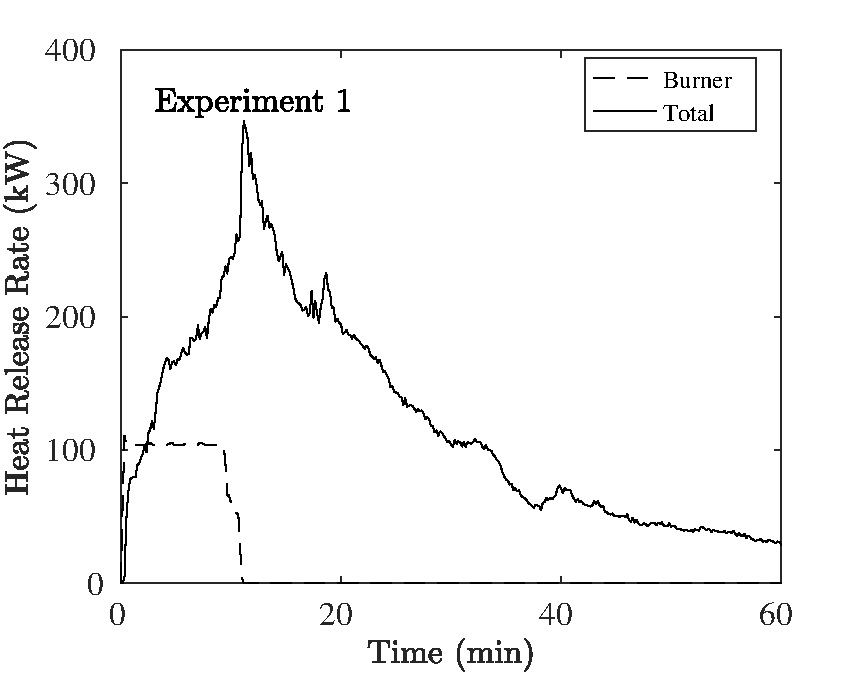
\includegraphics[height=2.15in]{../SCRIPT_FIGURES/Test_1_HRR} &
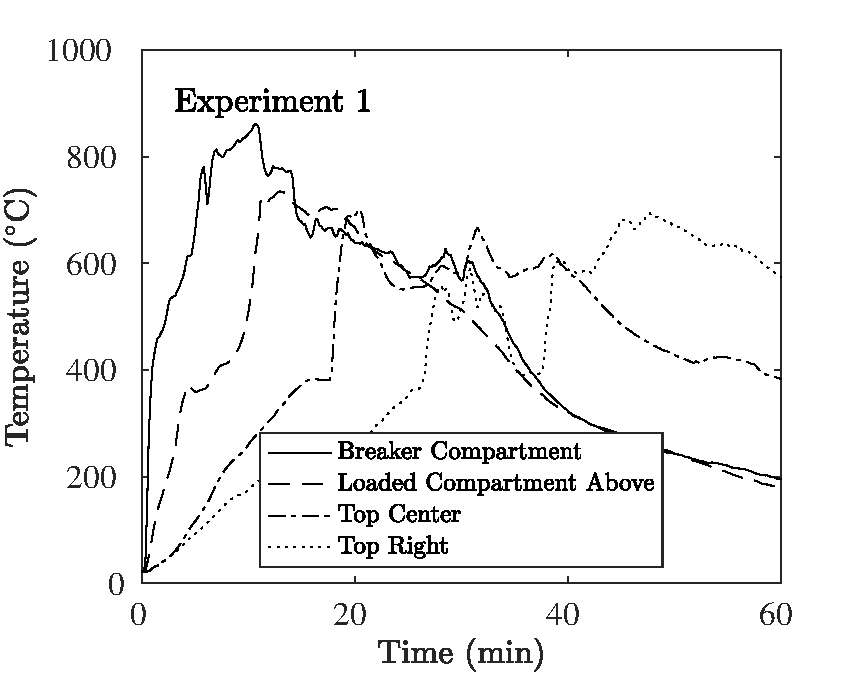
\includegraphics[height=2.15in]{../SCRIPT_FIGURES/Test_1_Gas_TC} \\
\multicolumn{2}{c}{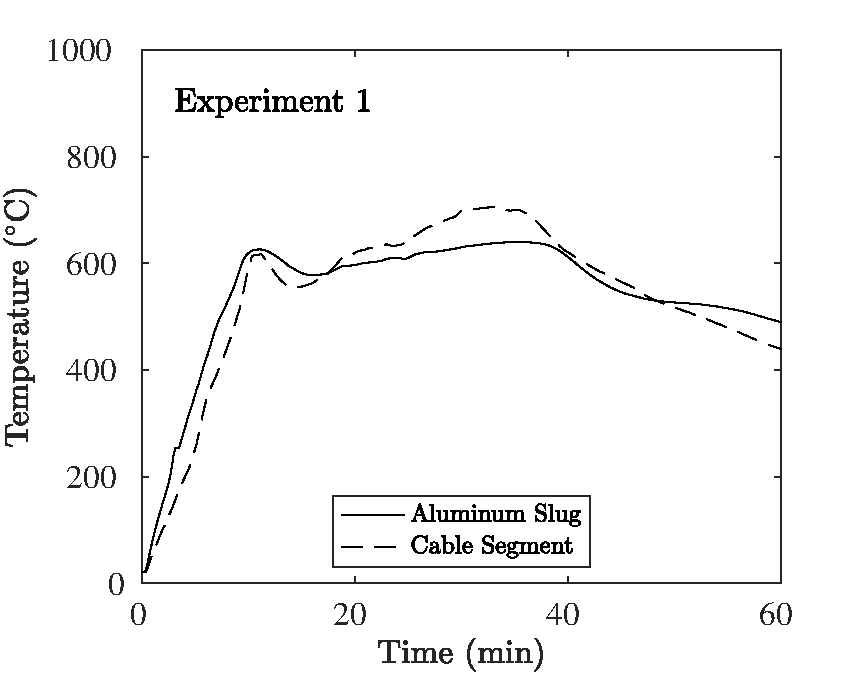
\includegraphics[height=2.15in]{../SCRIPT_FIGURES/Test_1_Slug_TC}}
\end{tabular*}
\caption[HRR and temperatures of Experiment 1]{Heat release rate (upper left), gas temperatures (upper right), and slug temperatures for Test~1.}
\label{fig:Test_1}
\end{figure}

\begin{figure}[p]
\centering
\includegraphics[height=2.5in]{../FIGURES/Test_1_9_min} \\
\includegraphics[height=2.5in]{../FIGURES/Test_1_17_min} \\
\includegraphics[height=2.5in]{../FIGURES/Test_1_47_min}
\caption[Photographs of Experiment~1]{Photographs of Experiment~1, 9~min, 17~min, and 47~min after ignition of the burner which was located in the lower left compartment.}
\label{fig:Test_1_photos}
\end{figure}



\clearpage

\subsection{Experiment 2}

The fire in Experiment~1 consumed all of the combustibles in the upper compartments of the large enclosure. However, the breakers in the center and right columns remained intact. For Experiment~2, the burner was placed beneath the right breaker with the aim of measuring its heat release rate with no other combustibles involved. The gas temperature in the compartment above the breaker reaches approximately 400~$^\circ$C, and there are no combustibles remaining from the previous experiment to sustain a fire.

\begin{figure}[!h]
\begin{tabular*}{\textwidth}{l@{\extracolsep{\fill}}r}
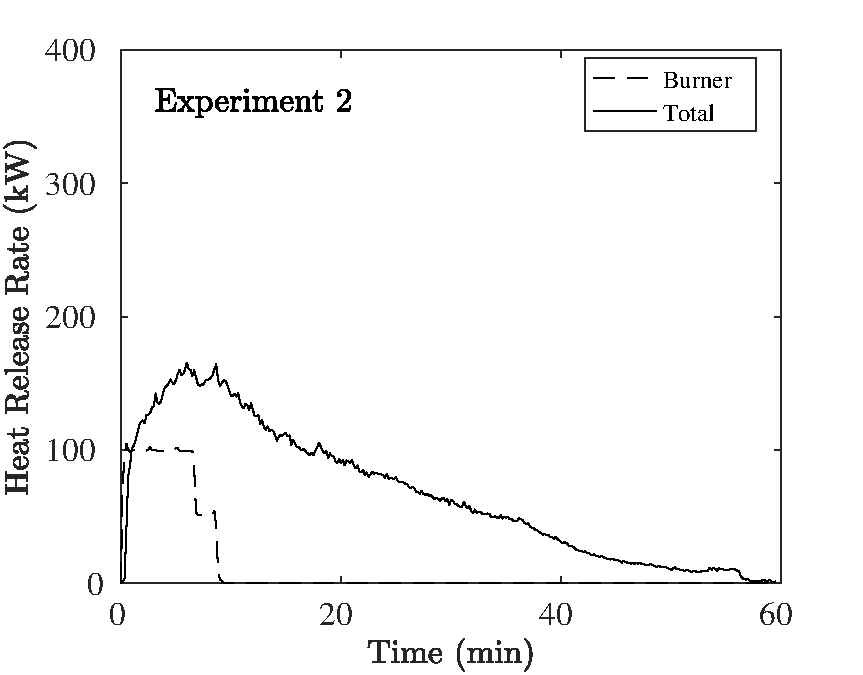
\includegraphics[height=2.15in]{../SCRIPT_FIGURES/Test_2_HRR} &
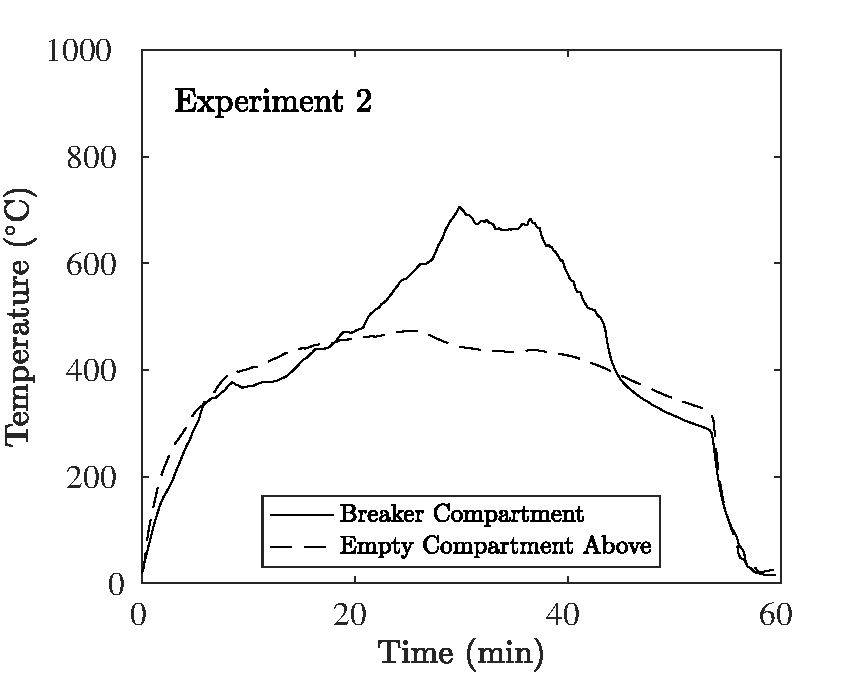
\includegraphics[height=2.15in]{../SCRIPT_FIGURES/Test_2_Gas_TC} \\
\multicolumn{2}{c}{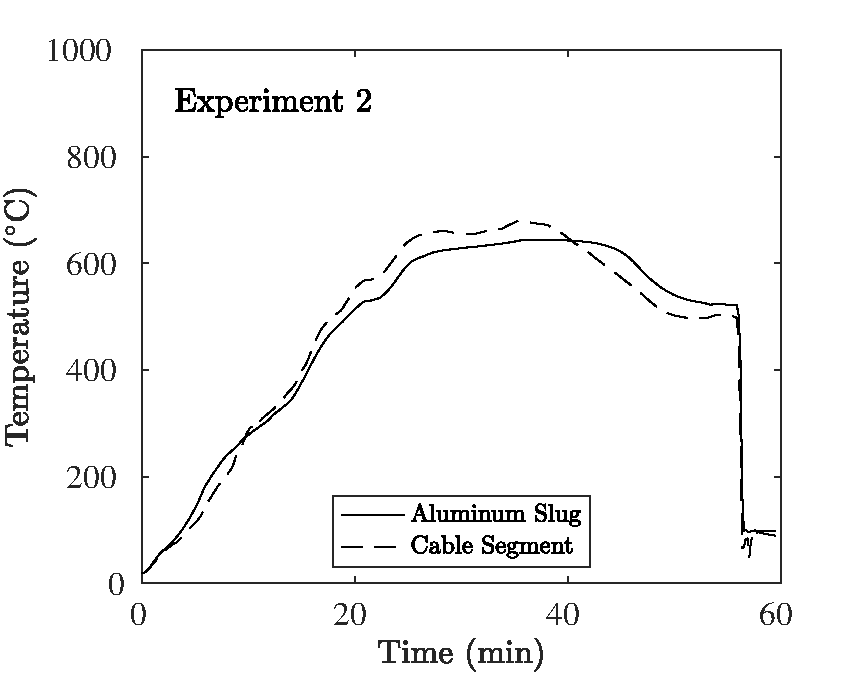
\includegraphics[height=2.15in]{../SCRIPT_FIGURES/Test_2_Slug_TC}}
\end{tabular*}
\caption[HRR and temperatures of Experiment 2]{Heat release rate (upper left), gas temperatures (upper right), and slug temperatures for Test~2.}
\label{fig:Test_2}
\end{figure}

\begin{figure}[p]
\centering
\includegraphics[height=2.5in]{../FIGURES/Test_2_15_min} \\
\includegraphics[height=2.5in]{../FIGURES/Test_2_30_min} \\
\includegraphics[height=2.5in]{../FIGURES/Test_2_60_min}
\caption[Photographs of Experiment~2]{Photographs of Experiment~2, 15~min, 30~min, and 60~min after ignition of the burner which was located in the lower right compartment. The bottom photograph shows the breaker after the experiment continues to glow red due to the heat trapped within.}
\label{fig:Test_2_photos}
\end{figure}


\clearpage

\subsection{Experiment 3}

This experiment was conducted within the single breaker enclosure, where the burner was positioned as in the previous experiments.

\begin{figure}[!h]
\begin{tabular*}{\textwidth}{l@{\extracolsep{\fill}}r}
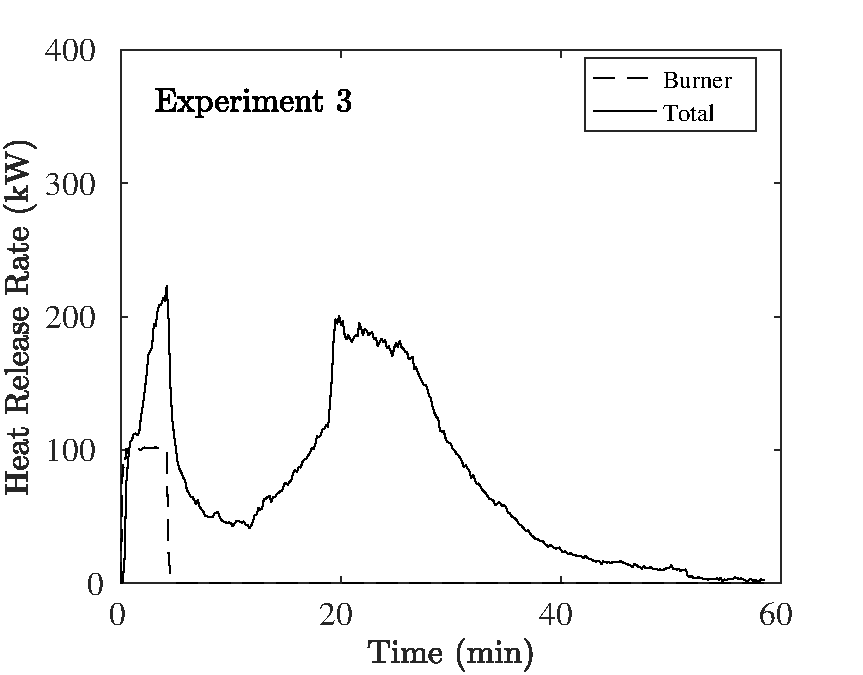
\includegraphics[height=2.15in]{../SCRIPT_FIGURES/Test_3_HRR} &
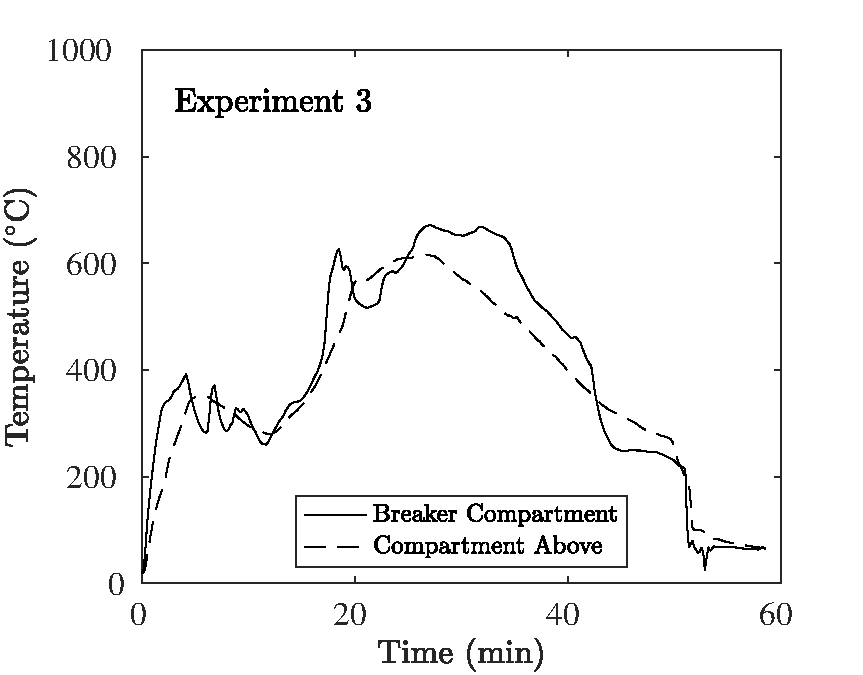
\includegraphics[height=2.15in]{../SCRIPT_FIGURES/Test_3_Gas_TC} \\
\multicolumn{2}{c}{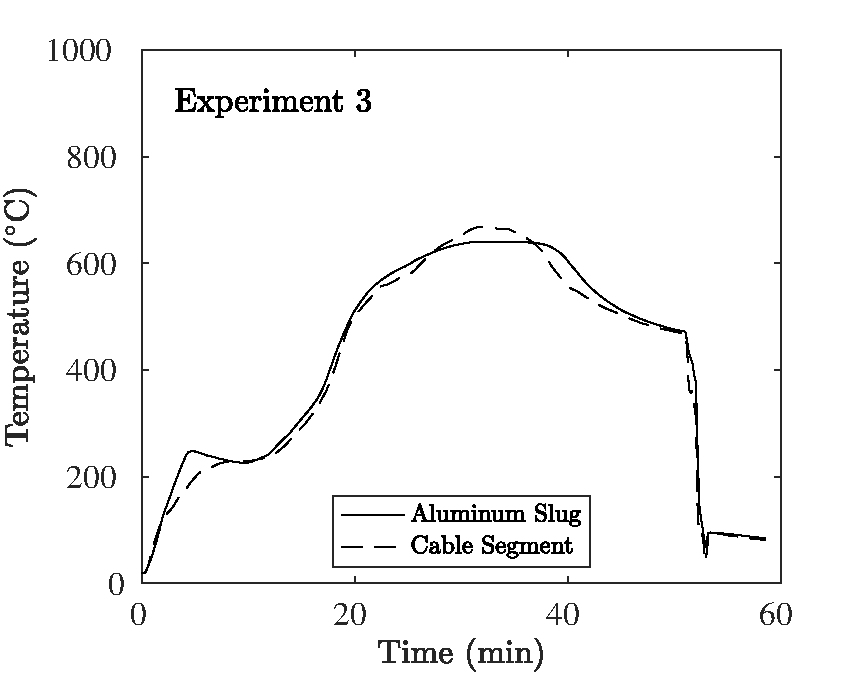
\includegraphics[height=2.15in]{../SCRIPT_FIGURES/Test_3_Slug_TC}}
\end{tabular*}
\caption[HRR and temperatures of Experiment 3]{Heat release rate (upper left), gas temperatures (upper right), and slug temperatures for Test~3.}
\label{fig:Test_3}
\end{figure}

\begin{figure}[p]
\centering
\includegraphics[height=2.5in]{../FIGURES/Test_3_8_min} \\
\includegraphics[height=2.5in]{../FIGURES/Test_3_19_min} \\
\includegraphics[height=2.5in]{../FIGURES/Test_3_39_min}
\caption[Photographs of Experiment~3]{Photographs of Experiment~3, 8~min, 19~min, and 39~min after ignition of the burner which was located in the lower compartment.}
\label{fig:Test_3_photos}
\end{figure}



\clearpage

\section{Conclusion}

Experiments were conducted to measure the heat release rates (HRR) and burning behavior of circuit breaker fires within closed steel enclosures. Of note:
\begin{itemize}
\item Fires within compartments of the enclosure resembled typical  ``flashover'' behavior; that is, flames emerging from the openings left behind after the instrument panels melted away. The measured temperatures within these compartments (both gas and solid) ranged between 600~$^\circ$C and 800~$^\circ$C, typical of an uninsulated steel enclosure.
\item In Experiment~1, the fire spread through double-walled steel partitions in approximately 10~min. Vigorous burning of combustibles was noted when the compartment gas temperature reached approximately 400~$^\circ$C.
\item The combustible load within the upper compartments was sufficient to maintain a fire long enough for the neighboring compartment to heat up and burn. 
\item The aluminum ``slug calorimeters'' and the interior of the instrumented cable segments exhibited similar temperatures, suggesting that the slugs might be a suitable surrogate to assess the vulnerability of electrical cables near or within a fire.
\end{itemize}



\section{Acknowledgment}

This research has been funded by the U.S. Nuclear Regulatory Commission, Office of Nuclear Regulatory Research, under the direction of Nicholas Melly and Gabriel Taylor.

Anthony Chakalis, Michael Selepak, Marco Fernandez, and Laurean DeLauter assisted in conducting the experiments.



\clearpage


\section*{References}
\addcontentsline{toc}{section}{References}
\bibliographystyle{unsrt}
\bibliography{FDS_general}





\end{document}
